\documentclass[../../course]{subfiles}

\renewcommand\thesection{\arabic{section}}


\begin{document}

\def\freqXOne{28}
\def\freqXTwo{28.1}
\def\freqXThree{56}

\section{Taking DTFT of the Complex Sequences} \label{sec:wrkTakingDTFTCplxSeqs}

In the previous section, we generated a bunch of \emph{Complex Sequences}. And
picked $4$ sequences for further analysis. In this section we will be taking
\textsc{DTFT} of these sequences. But before that, we need to take a look at what
a \textsc{DTFT} is and how to elagently compute it using python.

\subsection{Discrete Time Fourier Transform}

Discrete Time Fourier Transform, aka, \textsc{DTFT} transforms \emph{discrete time}
samples into a \emph{continous} signal in the \emph{frequency} domain. \textsc{DTFT}
is basically a special case of another transform known as \textsc{Z Transform}.
\textsc{Z Transform} can be mathematically described as,

\begin{align}
    X(z) = {\mathcal{Z}}\{x[n]\} = \sum_{n = - \infty}^{\infty} x[n] z^{-n}
\end{align}

where,

\begin{itemize} [label=]

    \item ${\mathcal{Z}}\{x[n]\}$: is the \textsc{Z Transform}.
    \item $x[n]$: is the input sequence, which was sampled with a
        particular \emph{sampling frequency}, $f_{s}$.
    \item $z$: is a \emph{complex number}, in the form $A e^{-j \omega}$.

        where,

        \begin{itemize} [label=]
            \item $A$: is the \emph{real part} or the \emph{amplitude}.
            \item $\omega$: is the \emph{complex argument} in radians.
        \end{itemize}

\end{itemize}

\textsc{DTFT} is a special case of \textsc{Z Transform}, where we take $A$
as $1$. Mathematically, we can describe \textsc{DTFT} as,

\begin{align}
    X(e^{j \omega}) &= X(z) |_{z = e^{j \omega}} \\
    &= \sum_{n = - \infty}^{\infty} x[n] z^{-n} \Big|_{z = e^{jw}} \\
    &= \sum_{n = - \infty}^{\infty} x[n] e^{-j w n} \label{eqn:dtftOmega}
\end{align}

Where $\omega$ can be substituted with $2 \pi f$, then the \textsc{DTFT} becomes,

\begin{align}
    X(e^{j 2 \pi f}) &= \sum_{n = - \infty}^{\infty} x[n] e^{-j 2 \pi f n}
    \label{eqn:dtftFreq}
\end{align}

Now eq. (\ref{eqn:dtftOmega}) becomes a function of \emph{frequency} $f$
instead of \emph{angular frequency} $\omega$. One thing to \textsc{note} is that,
\emph{sweeping} $f$ in eq. (\ref{eqn:dtftFreq}) from $0$ to $1$ will result in same
output as \emph{sweeping} $\omega$ in eq. (\ref{eqn:dtftOmega}) from $0$ to $2 \pi$.
Another interesting thing about \textsc{DTFT} is that the $e^{-1j \pi f n}$ will
\emph{scales} and \emph{wraps} the \emph{frequences} from $0$ to $\infty$ around
the \textsc{Unit Circle} in the $\mathcal{Z} \textsc{plane}$. Figure \ref{fig:wrapFreqUnitCircle}
attempts to visualizes this interesting concept.

\begin{figure}
    \centering
    \adjustbox{max width = 1\textwidth} {
        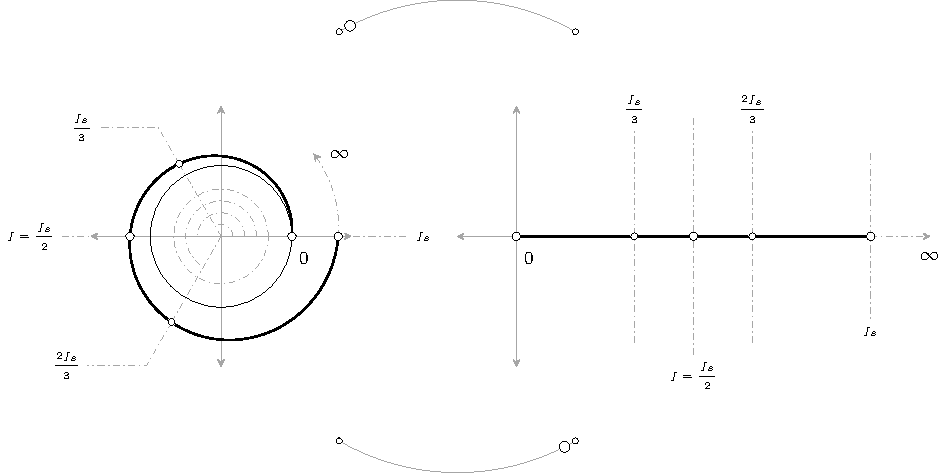
\includegraphics[height = 1\textheight] {tikzpics/epicWrapFreqUnitCircle.pdf}
    }
    \captionof{figure} {
        Wrapping frequencies around the \textsc{Unit Circle} in $\mathcal{Z}-\textsc{plane}$
    }
    \label{fig:wrapFreqUnitCircle}
\end{figure}



\subsection{Implementing DTFT using Python}

We essentially need to take \textsc{DTFT} of several\footnote{actually $4$, still
more than $1$} sequences. So it will be handy to implement a \emph{factory}, that
will take a \emph{sequence} and returns a \emph{dtft function} that can be called
with different \emph{frequences} and returns it's corresponding value. Let us call
this \emph{function} the \mintinline{python}{dtft_factory}.

%python/dtft_factory.py%
\begin{minted}[breaklines, autogobble, mathescape] {python}
    import numpy as np

    def dtft_factory(cplx_seq):

        def dtft(freq):
            sum = 0
            # see eq. ($\ref{eqn:dtftFreq}$)
            for n, cplx in enumerate(cplx_seq):
                sum = sum + cplx * np.exp(-1j * 2 * np.pi * freq * n)
            return sum

        return dtft

    seq = np.array([1, 1, 1, 1])
    dtft = dtft_factory(seq)

    print(type(dtft), end = "\n\n")

    print(dtft(0))
    print(dtft(1))

\end{minted}

\paragraph{Output}

\begin{minted}[breaklines, autogobble] {text}
    <class 'function'>

    (4+0j)
    (4+1.4695761589768238e-15j)
\end{minted}

Now, let's implement another \emph{function} that will \emph{mix}
and generate the \textsc{DTFT} for two given \emph{frequences}\footnote{one
as \emph{real} and one as \emph{complex}}. Another thing to note
is that the domain we need to evaluate. In the case of eq. (\ref{eqn:dtftOmega})
the \emph{}

% TODO: Finish this

Since the \textsc{DTFT} is
\emph{continous} in nature, let's take the sample count of the output
be $2000$.


%python/taking_dtft.py%
\begin{minted}[breaklines, autogobble, mathescape] {python}
    import numpy as np
    import matplotlib.pyplot as plt

    plt.figure(figsize = (6, 3))

    def dtft_factory(cplx_seq):

        def dtft(freq):
            sum = 0
            # see eq. ($\ref{eqn:dtftFreq}$)
            for n, cplx in enumerate(cplx_seq):
                sum = sum + cplx * np.exp(-1j * 2 * np.pi * freq * n)
            return sum

        return dtft

    ## $x_{1} + j x_{1}$

    def cplx_factory(samp_freq, real_freq, imag_freq):
        samp_period = 1 / samp_freq
        return lambda n: np.sin(
            2 * np.pi * real_freq * (n * samp_period)
        ) + 1j * np.sin(
            2 * np.pi * imag_freq * (n * samp_period)
        )


    N = 4024
    fs = 100
    cplx_fn = cplx_factory(fs, 10, 10.1)
    cplx_seq = np.ndarray(N, dtype = np.cdouble)

    for i in range(N):
        cplx_seq[i] = cplx_fn(i)

    freq = np.linspace(0.09, 0.12, 1000)
    dtft = dtft_factory(cplx_seq)
    dtft_seq = dtft(freq)

    plt.subplot(2, 1, 1)
    plt.plot(freq * fs, dtft_seq.real)

    plt.subplot(2, 1, 2)
    plt.plot(freq * fs, dtft_seq.imag)

    plt.savefig("../plots/deleme.pdf")

\end{minted}

\begin{figure}
    \centering
    \adjustbox{max width = 1\textwidth} {
        \includegraphics[height = 0.8\textheight] {plots/deleme.pdf}
    }
    \captionof{figure} {Some Figure}
    \label{fig:neverMind}
\end{figure}



%% In Sections \ref{sec:wrkGenSeqs} and \ref{sec:wrkGenCompSeqs}, we did

%%% A
%%% $x_{1} + j x_{1}$
%
%\textbf{Sequence:} $\sin(2 \pi \freqXOne t) + j \sin(2 \pi \freqXOne t)$
%
%%% B
%%% $x_{1} + j x_{2}$
%
%\textbf{Sequence:} $\sin(2 \pi \freqXOne t) + j \sin(2 \pi \freqXTwo t)$
%
%%% C
%%% $x_{1} + j x_{3}$
%
%\textbf{Sequence:} $\sin(2 \pi \freqXOne t) + j \sin(2 \pi \freqXThree t)$
%
%%% F
%%% $x_{2} + j x_{3}$
%\textbf{Sequence:} $\sin(2 \pi \freqXTwo t) + j \sin(2 \pi \freqXThree t)$
%
%%%  a, b, c, f


\end{document}
